\newpage
\section{MapReduce}
\label{sec:mapreduce}

\noindent
It's 2004 and Google is looking for a way to process large amounts of web-crawled data efficiently in parallel.
They found that most jobs follow the same pattern, leading to the following model:
\begin{Def}[MapReduce]

    \textbf{MapReduce} automatically parallelizes and executes client jobs provided they give these two functions:
    \begin{itemize}
        \item \textbf{Map}: Takes a set of input key-value pairs and produces a set of intermediate key-value pairs.
        \item \textbf{Reduce}: Takes an intermediate key and a set of values for that key, and merges them into a smaller set of values.
    \end{itemize}
\end{Def}

\begin{Note}
    If you are familiar with functional programming, the MapReduce model is similar to the \texttt{map} and \texttt{reduce} functions as seen in languages like Python or JavaScript.
\end{Note}

\begin{Example}[Word Count in MapReduce]

    \label{ex:wordcount}
    \noindent\textbf{Input:} A collection of documents (each document has a name and contents).\\
    \noindent\textbf{Output:} The total frequency of each word across all documents.\\[0.5em]

    \noindent\textbf{Map:}
    \begin{itemize}
      \item \textbf{Key:} document name  
      \item \textbf{Value:} document contents  
      \item \textbf{Emit:} for each word \(w\) in the document, emit \((w,1)\), of form (key, value)
    \end{itemize}

    \noindent\textbf{Reduce:}
    \begin{itemize}
      \item \textbf{Key:} a word \(w\)  
      \item \textbf{Value:} list of counts \(\{1,1,\dots,1\}\) from all maps  
      \item \textbf{Emit:} \(\bigl(w,\sum \text{counts}\bigr)\), i.e.\ the total occurrences of \(w\)
    \end{itemize}

    \noindent\textbf{Example:} \{($A$, ``the dog likes to sit''), ($B$, ``the lion does not sit'')\}
    maps to\\
    \{(the, 1), (dog, 1), (likes, 1), (to, 1), (sit, 1), (the,1) (lion, 1), (does, 1), (not, 1),(sit,1)\}\\[0.5em]
    This is then reduced to,\\
    \{(the, 2), (sit, 2), (dog, 1), (likes, 1), (to, 1), (lion, 1), (does, 1), (not, 1)\}.
\end{Example}

\newpage 

\noindent
We can even stack multiple MapReduce jobs together. For example consider the below figure based on trying to find the 
set difference in Example (\ref{ex:wordcount}):

\begin{figure}[h]
    \centering
    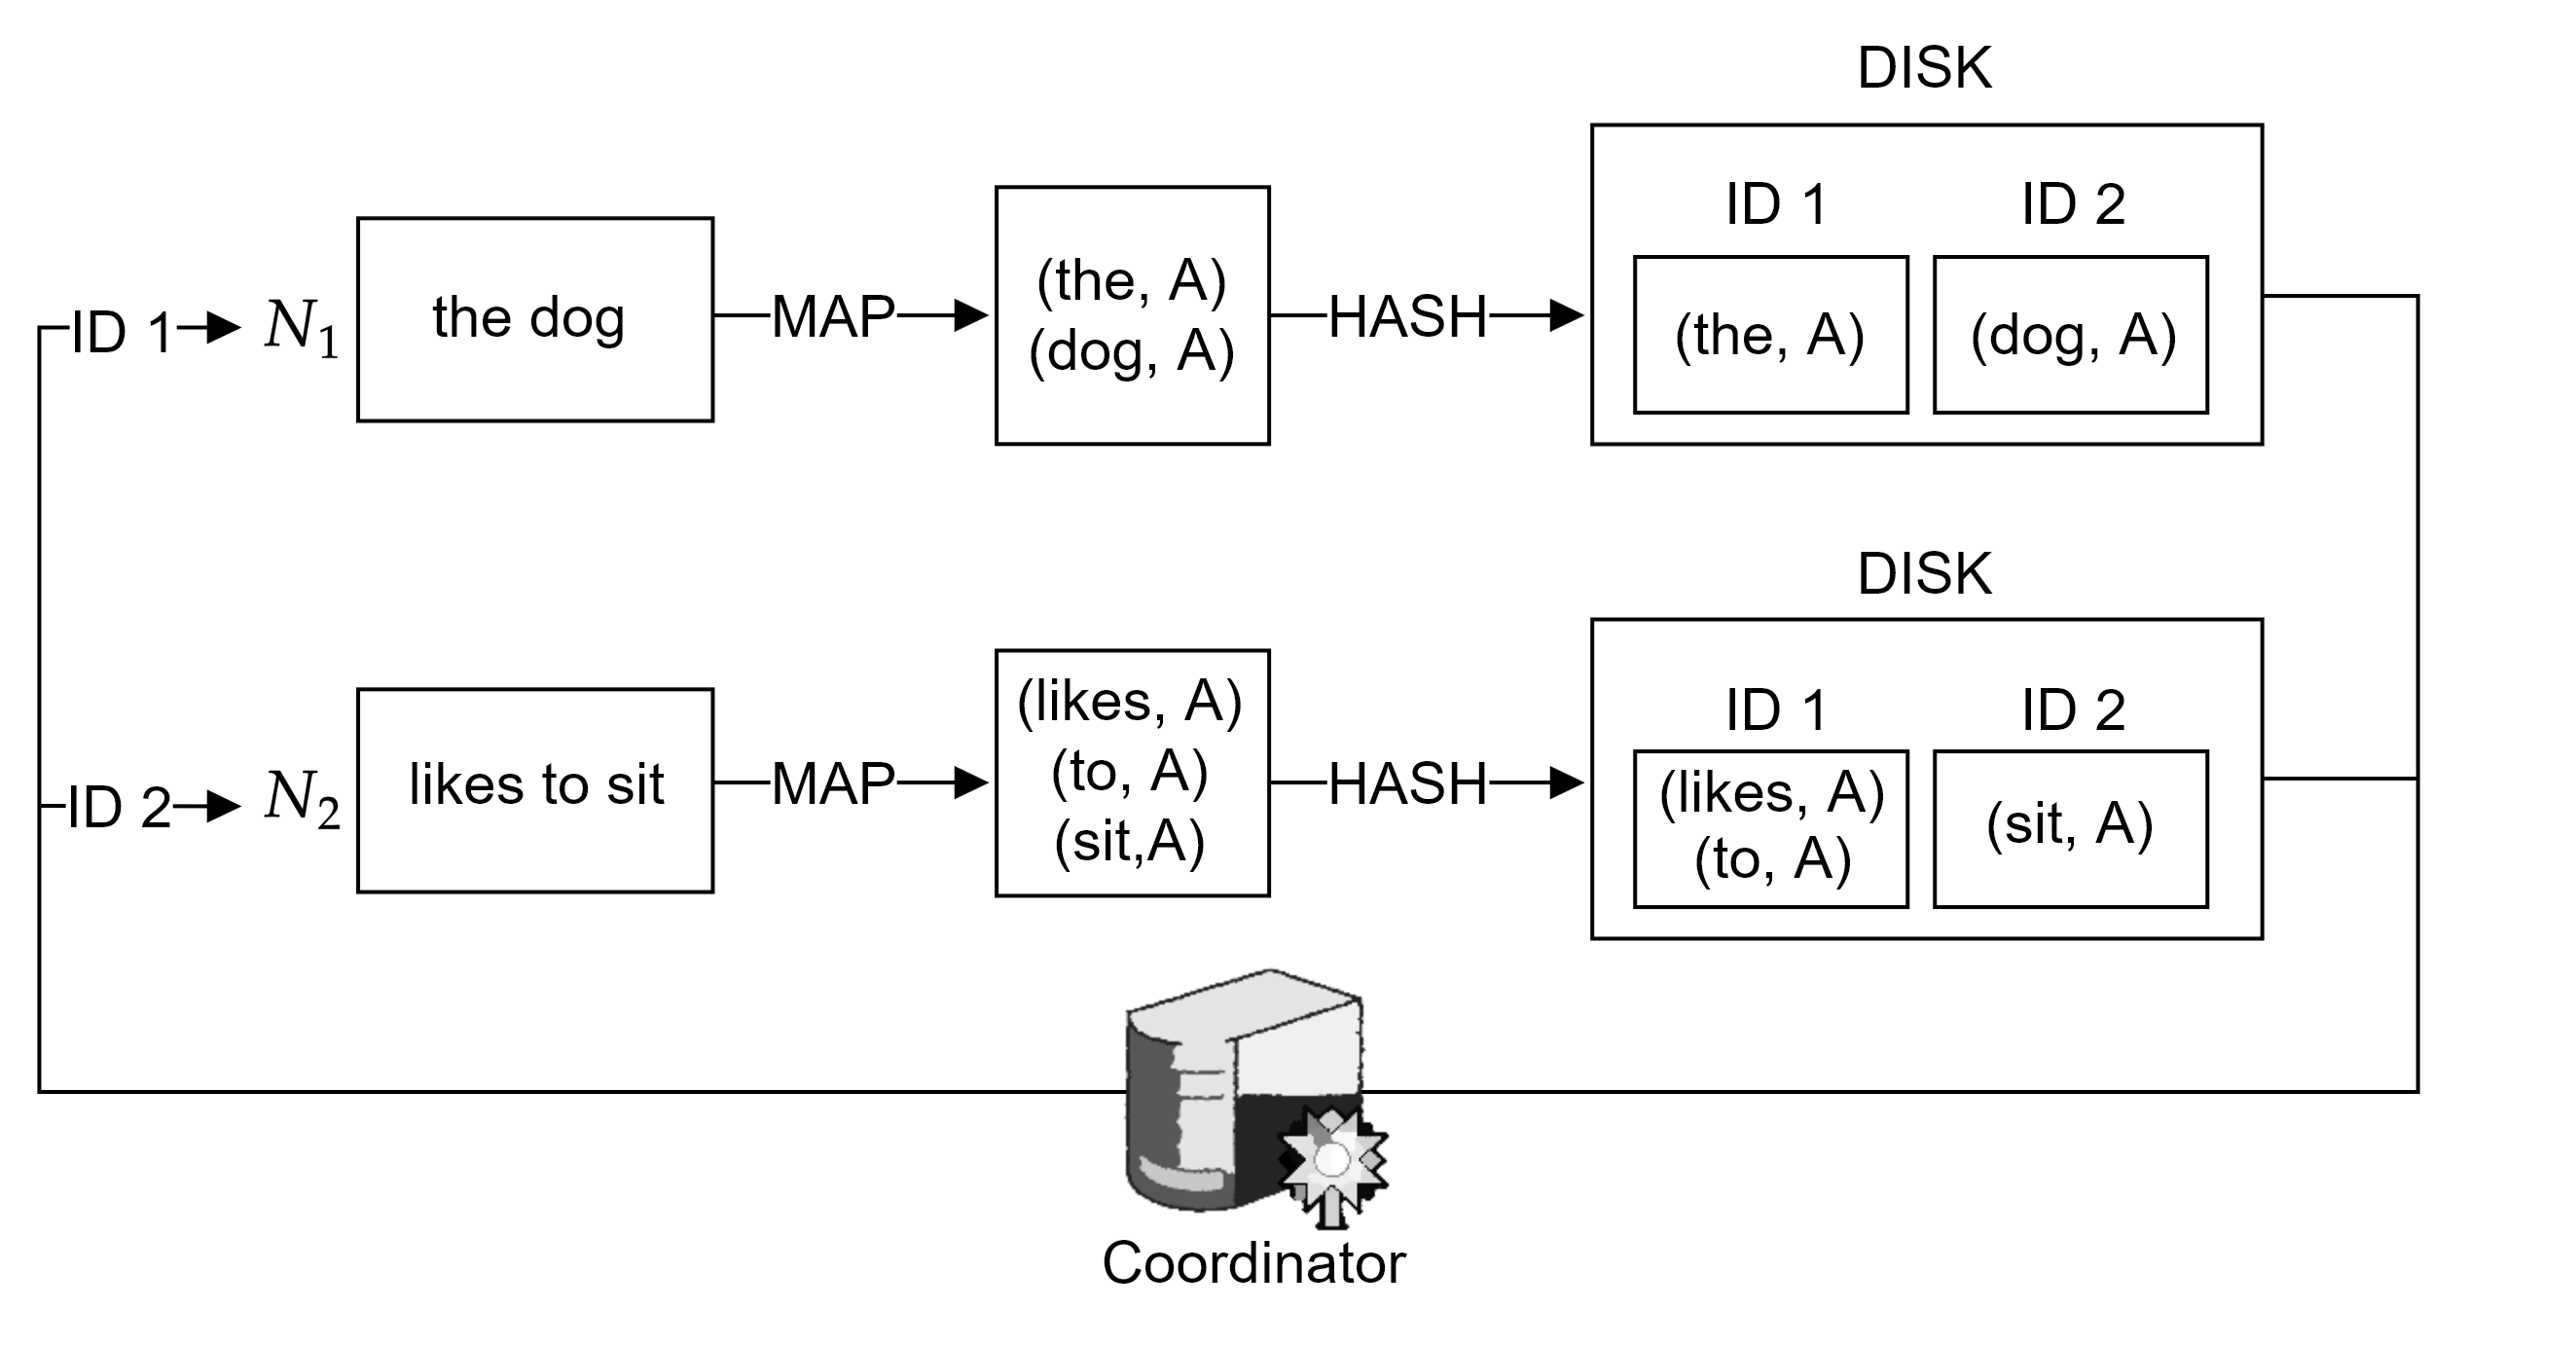
\includegraphics[width=\textwidth]{Sections/mapreduce/multi.png}
    \caption{Both sets $A$ and $B$ under going two rounds of MapReduce. The first creates a set of words between $A$ and $B$. The 
    second round discards non-singletons, reducing the set to counts of elements in $A$ and $B$.}
    \label{fig:mapreduce}
\end{figure}

\noindent
Now to bring this into a distributed system:

\begin{Def}[Implementing MapReduce in a Distributed System]

    To implement MapReduce with a single coordinator as follows:
    \begin{itemize}
        \item \textbf{Split Data}: First take the input data and split it into $M$ chunks.
        \item \textbf{Assign Maps}: The coordinator distributes the $M$ chunks to $N$ worker nodes (may receive multiple chunks).
        \item \textbf{Map Phase}: Each worker processes its chunk and partitions the output into $R$ sections on disk. This is 
        achieved by uniformly hashing the intermediate keys into $R$ buckets.
        \item \textbf{Shuffle Phase}: The coordinator collects the $R$ partitions from all workers and redistributes them back to $N$ workers, via 
        sorting the intermediate keys, or by hashing (more efficiently).
        \item \textbf{Reduce Phase}: Each worker processes its partition and writes the final output to disk.
    \end{itemize}

    \noindent
    Additionally, Given $W$ workers, $M$ mapping tasks, and $R$ reducing tasks, $W \gg N$ and $R \gg N$. I.e.,
    Mapping and Reducing tasks should outnumber the workers to keep them busy.
\end{Def}

\newpage 
\noindent
Now to deal with failures:

\begin{Def}[Fault Tolerance in MapReduce]

    We deal with hiccups in our system via the following:
    \begin{itemize}
        \item \textbf{Map/Shuffle Phase}: If a worker fails to map or goes offline with the intermediate data, the coordinator will reassign the chunk to another worker.
        \item \textbf{Reduce Phase}: If a worker fails to reduce, the coordinator will reassign the partition to another worker.
        \item \textbf{Coordinator Failure}: If the coordinator fails, the system will need to restart the entire MapReduce job. Failures are not recoverable, and are assumed to be rare.
    \end{itemize}
\noindent
    If a worker is slow (\textbf{straggler}), the coordinator reassigns its task and reacts accordingly:
    \begin{itemize}
        \item \textbf{Map Phase}: The coordinator will only point to the first worker that finishes the map task for intermediate data.
        \item \textbf{Reduce Phase}: It doesn't matter who finishes first, as they write the same data to the same location on disk (e.g, ``/filepath/final\_data/id''). Moreover, writing is atomic.
    \end{itemize}
\end{Def}

\begin{figure}[h]
    \centering
    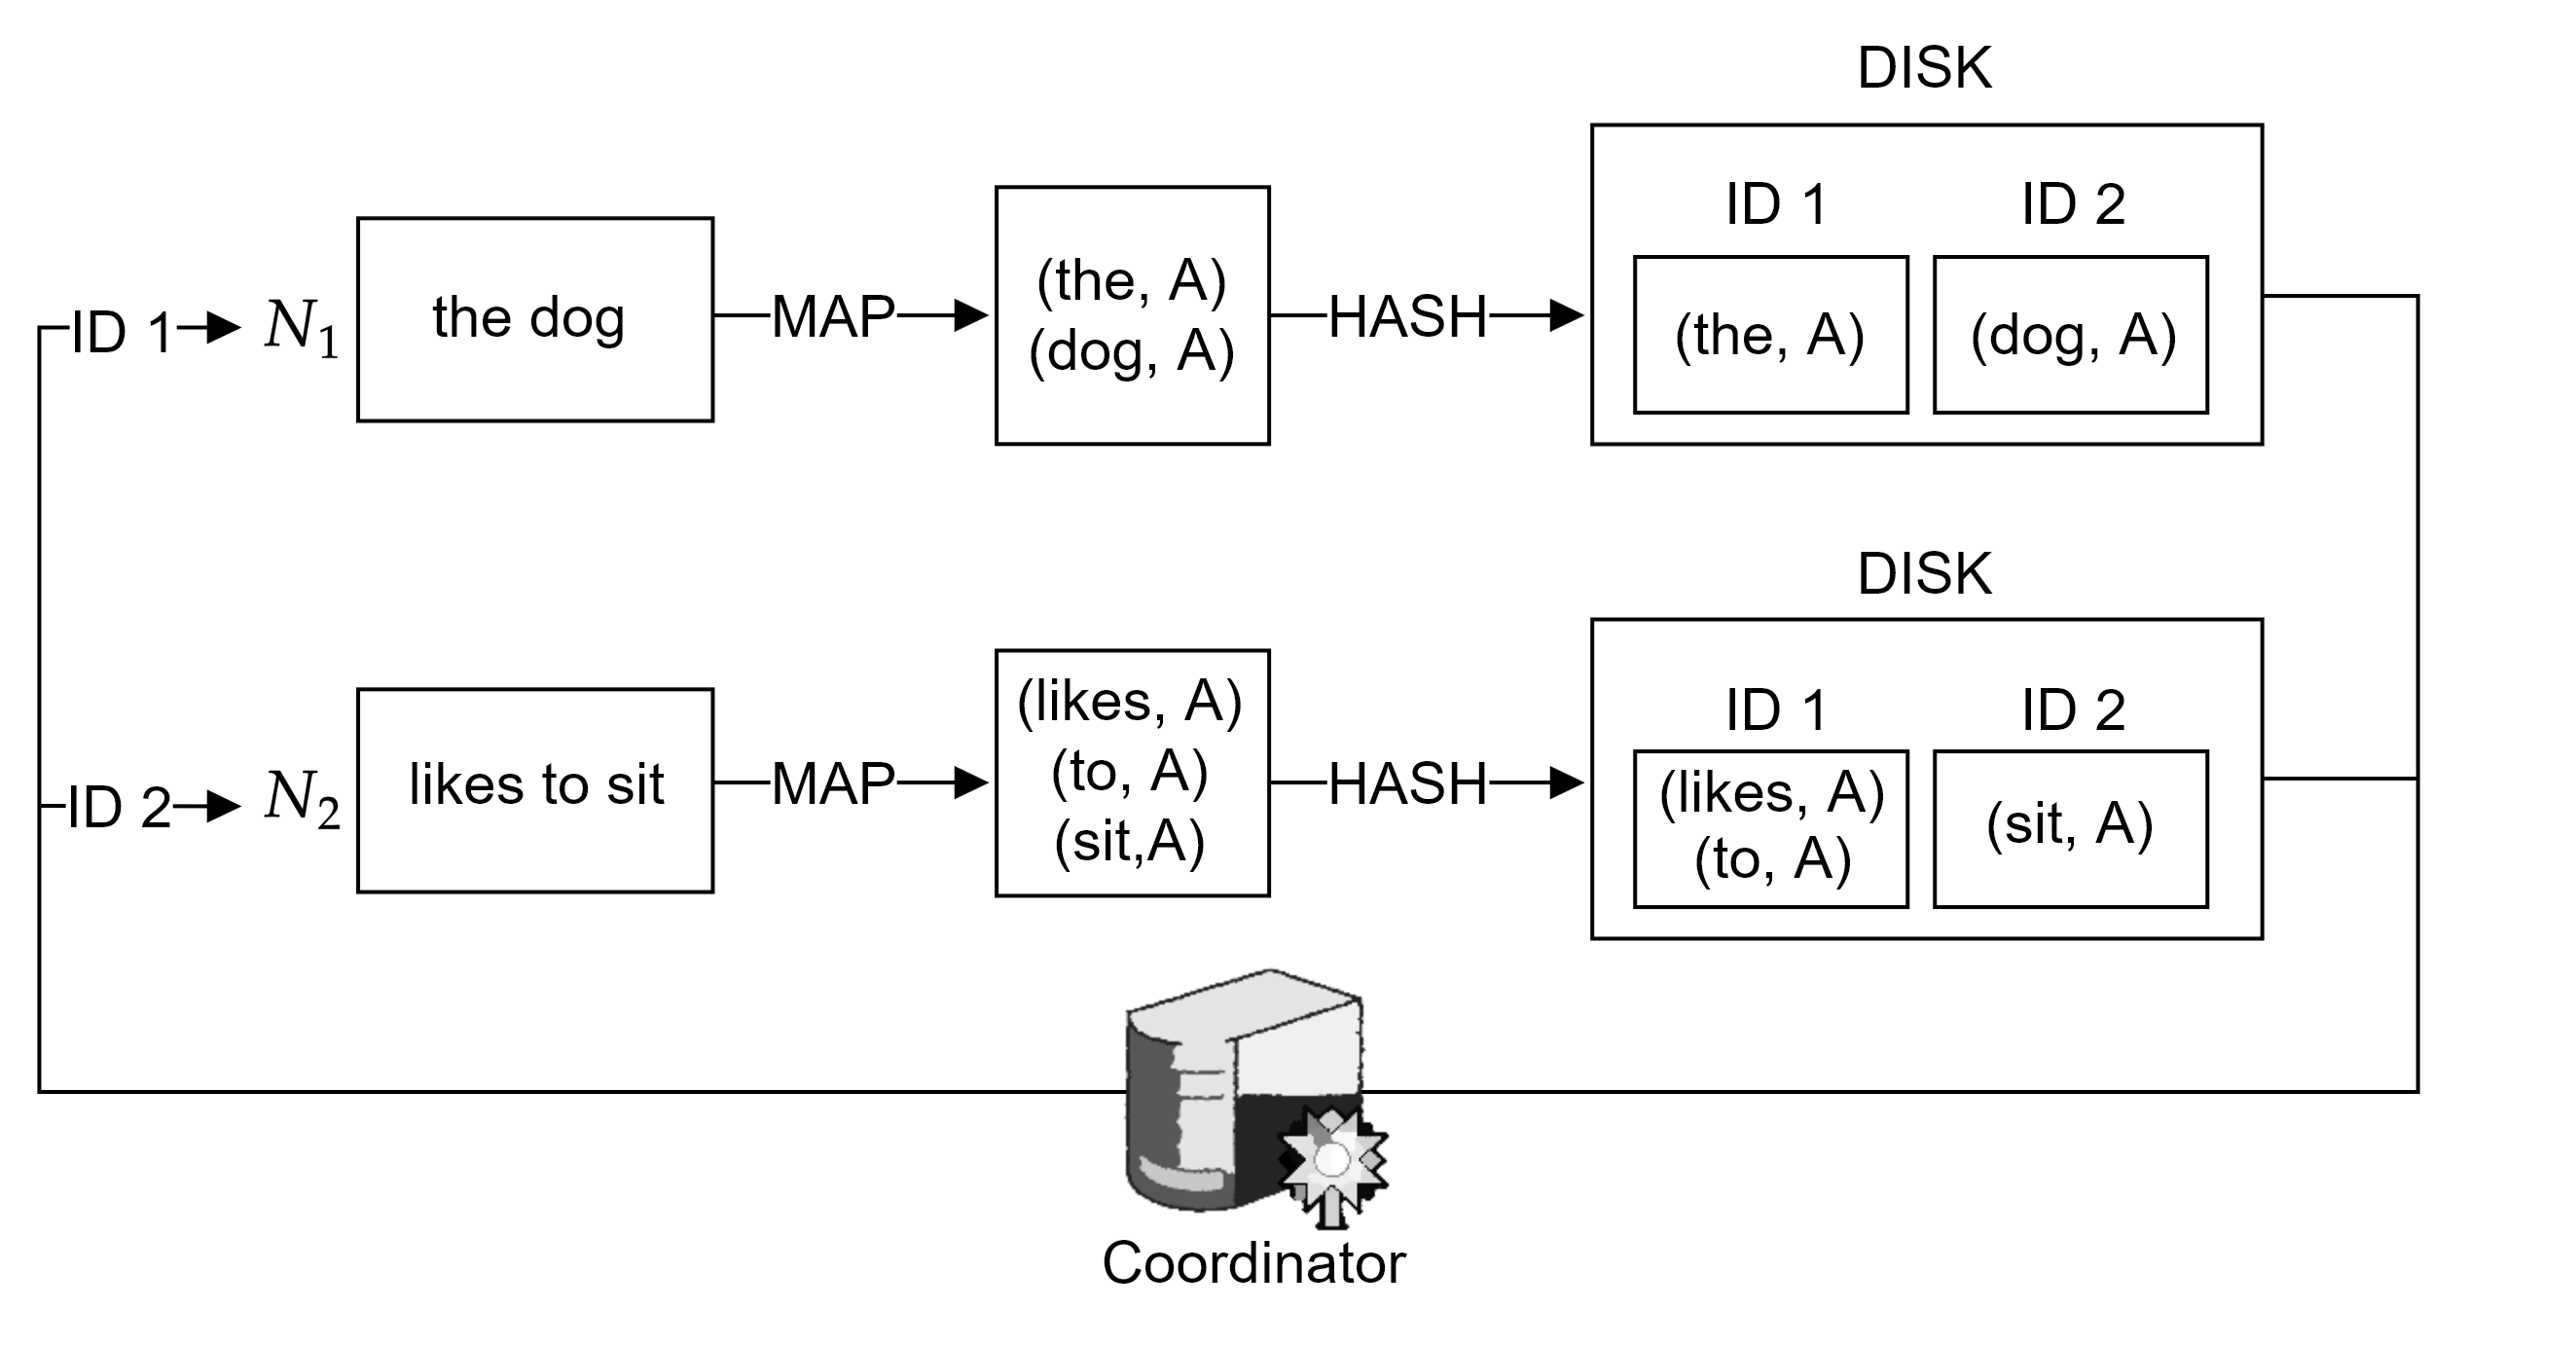
\includegraphics[width=\textwidth]{Sections/mapreduce/nwork.png}
    \caption{In a simplified MapReduce system, two workers receive a partitioned map job of ``the dog likes to sit". After $N_1$ and $N_2$ finish 
    processing the job, they hash the intermediate data into $R=2$ buckets. The coordinator then collects the buckets assigning ID 1$\to N_1$ and ID 2$\to N_2$, to finish the reduce job.}
    \label{fig:nwork}
\end{figure}


